% -*- mode: latex; mode: auto-fill -*-
\chapter{User Description of GASP}

\section{Introduction}

This chapter gives an overview of GASP aimed at people who wish
to use the existing functionality provided by GASP.

As GASP makes use of the graphics capabilities of the \XGAP{} share
package, the user must start \XGAP{} in order to use the system.  This
is achieved by running the \texttt{xgap} command at the shell prompt.
After \XGAP{} has started and \texttt{gap>} prompt is shown, GASP must
be loaded.  This is achieved with the \texttt{RequirePackage} command:
\begin{verbatim}
gap> RequirePackage("gasp");
true
\end{verbatim}

\noindent Here, the lines that do not start with \texttt{gap>}
represent the output from \GAP{}.  At this point, the user may start
using GASP.

\section{An Example of GASP}

To get a feeling of how to use GASP, it is best to look through an
example.  The following example brings up a window from which the user
can simulate the Strauss Process using the Metropolis-Hastings
algorithm.  The example demonstrates setting up the algorithm for use
with the simulation framework, and observing the behaviour through the
\emph{graphical user interface} (GUI).

\begin{verbatim}
gap> # create a 300x300 configuration of points
gap> config := PointConfiguration(0,0,300,300);
PointConfiguration( 0, 0, 300, 300 )
gap> # create the appropriate proposal function
gap> propose := CreateSimpleFlipPropose(1/2);
function( cnf ) ... end
gap> # create the appropriate acceptance check function
gap> check := CreateStraussCheck(1/900, 9/10, 15);
function( cnf, change ) ... end
gap> # create a window to run the simulation in
gap> GUISimulate(config, "Strauss", 300, 300, propose, check);
<graphic sheet "Strauss">
\end{verbatim}

First we create an object \texttt{config} to hold the state of the
simulation, which is a configuration (ie. finite, unordered list) of
points on the plane.  Next, proposal and acceptance check functions
for the desired algorithm are created.  The exact use of these is
covered in Section \ref{sect:sim-framework}.

Finally, we invoke the GASP command \texttt{GUISimulate}, which brings
up a window from which we can observe what is going on.  We also tell
\GAP{} to output log messages from the simulation to the console.  The
window should look similar to the one in Figure
\ref{fig:strauss-screenshot}.  The screen shot differs from the window
initially shown by \texttt{GUISimulate} because the simulation has
been running for a few iterations.

\begin{figure}[hbt]
\centering
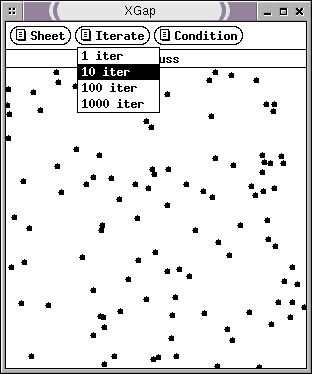
\includegraphics{strauss}
\caption{The simulation display window}
\label{fig:strauss-screenshot}
\end{figure}

\section{Using the Graphical User Interface}

The \emph{graphical user interface} (GUI) offers a nice way to
experiment with the simulation framework.  It is the window displayed
when \texttt{GUISimulate} is called, as shown in Figure
\ref{fig:strauss-screenshot}.  The main area of the window displays
the current state of the algorithm.  In the example, the display area
starts out empty, and as the simulation runs, it fills up with points.

There is a menu bar along the top of the window, from which a user
can control the simulation.  The first item on the menu bar is the
standard \XGAP{} `Sheet' menu.  It contains menu items to save the
contents of the display area as a postscript file, and to close the
window.

The second item opens the `Iterate' menu, which is specific to GASP.
It contains options to let the simulation run for various numbers of
iterations.  The display area updates after the desired number of
iterations have been made.

In some cases, running the simulation for a particular number of
iterations is not what is desired.  Sometimes a user may want to run
the simulation until a particular event occurs.  This can be achieved
with the `Condition' menu.  (To understand the condition menu fully,
see Section \ref{sect:sim-framework} which describes the simulation
framework).  The conditions in the `Condition' menu on which GASP can
pause the simulation are:

\begin{description}
\item[\emph{Until first acceptance}] iterates until a proposition is
accepted, after which the simulation stops.
\item[\emph{Until first acceptance $($max 100 iter$)$}] is like above,
but also stops if 100 iterations are made without an acceptance.  This
option is useful in cases where it is not guaranteed that a
proposition will ever be accepted.
\item[\emph{Until first rejection}] iterates until a proposition is rejected,
after which it stops.
\item[\emph{Until first rejection $($max 100 iter$)$}] is like above,
but also stops if 100 iterations are made without a rejection.
\item[\emph{Until propose add object $($max 100 iter$)$}] iterates
until we get an `add object' proposal, or 100 iterations are made,
whichever comes first
\item[\emph{Until propose delete object $($max 100 iter$)$}] iterates
until we get a `de\-lete object' proposal, or 100 iterations are made,
whichever comes first.
\end{description}


\section{General Framework Used in Simulations}\label{sect:sim-framework}

GASP provides a generic framework for running certain algorithms that
can be expressed according to the flowchart describing the framework
shown in Figure \ref{fig:flowchart}.

\begin{figure}[hbtp]
\centering
\includegraphics[width=4in]{simulate-flowchart}
\caption{Simulation flow of control}
\label{fig:flowchart}
\end{figure}

The framework can also be described by the following set of rules:

\begin{enumerate}
\item propose a change to the current configuration.
\item calculate the acceptance probability for this proposed change.
That is, the probability of applying the proposed change.
\item make a random decision whether to accept or reject the proposed
change according to the acceptance probability calculated in step 2.
\begin{itemize}
\item if it is accepted, apply the proposed change to the configuration.
\item if it is rejected, discard the proposed change.
\end{itemize}
\item check to see if the simulation should continue.  If so, go to
step 1 and repeat.  If not, then the simulation stops.
\end{enumerate}

The GASP simulation framework can run multiple types of algorithms.
The different algorithms are defined by the combination of a
\emph{proposal} function and an \emph{acceptance check} function.
These two functions are passed to the \texttt{GUISimulate} function in
order to run the algorithm.

In the case of the Strauss Process example above, we used a very
simple proposal function which would either propose adding a random
new point or removing a random existing point, with equal probability.
Instead of writing the implementation of this function in full in the
example, we used the \texttt{CreateSimpleFlipPropose} command, which
returns a proposal function which adds a point with the desired
probability.

For the acceptance check function, we want to use the reference
formula used when simulating the Strauss Process with the
Metropolis-Hastings algorithm, except that we calculate it in terms of
the proposed next state, rather than the current one.  Once again, we
use a convenience function to implement this:
\texttt{CreateStraussCheck}.  This function returns the appropriate
acceptance check function.

The other parameters passed into the main simulation function
\texttt{GUI\-Simulate} are the \texttt{Configuration} object, a
continue checking function and optionally a file to log the progress
of the simulation.  The configuration object is simply the object that
holds the state of the simulation.  This is mainly the collection of
objects (such as points) that make up the configuration.  In the
Strauss process example above, we used the \texttt{PointConfiguration}
that is part of GASP as described in Section
\ref{sect:configurations}, which represents a configuration of points.

Deciding whether or not to continue the simulation is controlled from
the GUI through the `Iterate' and `Condition' menus.  More specialised
control over deciding whether to continue is possible, provided the
user is willing to write some simple \GAP{} code.

It is possible to log the progress of the simulation if desired.  This
is achieved through the seventh optional argument to
\texttt{GUISimulate}.  To send the log messages to the \GAP{} console,
the user can pass \texttt{OutputTextUser()} as this argument.  To
append log messages to the file \emph{filename}, the user can pass
\texttt{OutputTextFile(\emph{filename}, true)} as the argument.  If
the argument is omitted, then log messages are not recorded.


\section{Predefined Functionality}

GASP supports a number of \texttt{Configuration} object types and
provides several proposal and acceptance check functions.  If the
algorithm the user is interested in is supplied by GASP, then it is
very easy to use GASP.

\subsection{Configurations}\label{sect:configurations}

A configuration object stores all information about the current state
of a simulation.  At a minimum, this is a collection of objects in the
state, but may hold more information.

Configurations implement a number of operations that can be used to
manipulate them (for example, counting how many objects are in the
configuration or choosing a random object in the configuration).  This
makes it possible to implement algorithms that are independent of the
actual configuration type used.

Currently, GASP provides configuration implementations for use in both
point process and line process simulations.  These are called the
\texttt{Point\-Configuration} type and \texttt{Line\-Configuration}
type.

The \texttt{Point\-Configuration} object can be created using the
following command:
\begin{lstlisting}{}
config := PointConfiguration(sx,sy, swidth,sheight);
\end{lstlisting}

\noindent The first four parameters specify the top left corner
(assuming the origin is in the top left corner of the GUI window,
consistent with the coordinate system used for the computer screen)
and the dimensions of the region the simulation will occur in.

The \texttt{LineConfiguration} object can be created in a similar
fashion:
\begin{lstlisting}{}
config := LineConfiguration(sx,sy, swidth,sheight);
\end{lstlisting}

\noindent The parameters have the same meaning as for
\texttt{PointConfiguration}.

\subsection{Proposal Functions}

The proposal function for a particular algorithm is responsible for
proposing changes to the state of a configuration.  Given the current
state of a configuration, it will return a proposed change (for
example, adding a point).  Usually it takes into account the current
state of the configuration, but may also use the iteration number,
some other counter or the output of a random number generator to
decide on the proposal.  GASP provides a number of predefined proposal
functions that may be useful for the user's simulation.

As most proposal functions have several parameters, it could
potentially be time consuming to rewrite the function each time the
user wanted to change a parameter.  To save time, \emph{function
factories} are provided for the proposal functions that GASP provides.
Function factories are simply functions that return functions.  These
factories provide an easy way to create members of families of
proposal functions.

\subsubsection{CreateSimpleFlipPropose}

\texttt{CreateSimpleFlipPropose} creates proposal functions that
choose between adding a randomly placed new point or removing an
existing point at random.  The probability of proposing to add a new
point is passed in as a parameter to \texttt{CreateSimpleFlipPropose}.
A proposal function of this type can be created like this:
\begin{lstlisting}{}
propose := CreateSimpleFlipPropose(prob);
\end{lstlisting}

\noindent In the case that there are no points in the configuration,
this proposal function always proposes to add a new point.  This
proposal function is appropriate for point processes using the
Metropolis-Hastings algorithm.

\subsubsection{CreateRedBlackPropose}

\texttt{CreateRedBlackPropose} creates a proposal function that
implements the Widom-Rowlinson `Red-Black' point process as described
in Section \ref{sect:widom-rowlinson}.  For a full
description of how the Widom-Rowlinson process is implemented in the
GASP simulation framework, see the example in Section
\ref{sect:red-black-example}.

The user can create the proposal functions of this type with the following
command:
\begin{lstlisting}{}
propose := CreateRedBlackPropose(radius, mean_red,
                                 mean_black);
\end{lstlisting}

\noindent The first argument is the minimum required distance between
points of different colours.  The second is the mean for the Poisson
distribution that is used to select the number of red points to add in
one phase of the simulation.  The third argument plays a similar role
for the black points.

\subsection{Acceptance Check Functions}

The acceptance check function for an algorithm is responsible for
calculating the probability of accepting the proposed new state for
the configuration.  This decision will generally be made based on the
current and proposed change.  Based on the probability calculated by
the acceptance check function, GASP will make a random decision
whether or not to accept the proposed change.

There are a number of check functions provided with GASP.  Similar to
the proposal functions, factories are provided to make experimentation
more convenient.

\subsubsection{CreateStraussCheck}

The function \texttt{CreateStraussCheck} creates acceptance check
functions that implement the formula for the acceptance probability
for the Strauss Process.  The user can create a Strauss process
acceptance check function with the following command:
\begin{lstlisting}{}
check := CreateStraussCheck(beta, gamma, radius);
\end{lstlisting}

\noindent The arguments \emph{beta} and \emph{gamma} passed to this
function are the $\beta$ and $\gamma$ parameters in the density
function, and \emph{radius} is the distance $r$, used when calculating
$s(\mathbf{x}, y)$, as described in Section
\ref{sect:strauss-process}.

%\emph{XXXX - it would probably be good to have a general MH check
%function that just took the density function for the desired distribution}

\subsubsection{CreateFixedCheck}

The function \texttt{CreateFixedCheck} creates an acceptance check
function that always returns a particular probability regardless of
the current state or proposed change.  This type of acceptance check
function may be created with the following command:
\begin{lstlisting}{}
check := CreateFixedCheck(prob);
\end{lstlisting}
\noindent For this function, \emph{prob} is the probability that is
returned.

\subsection{Problems Covered}

By combining a proposal function and an acceptance check function as
arguments to \texttt{GUISimulate}, a number of algorithms can be
simulated when passed to \texttt{GUISimulate}.  As seen in the example
at the start of the chapter, \texttt{CreateSimpleFlipPropose} and
\texttt{CreateStraussCheck} can be used to simulate a Strauss Process
using the Metropolis-Hastings Algorithm.

The \texttt{CreateRedBlackPropose} and \texttt{CreateFixedCheck}
functions can be combined to simulate the Widom-Rowlinson point
process.  In this case, we use a probability of 1 as the parameter
for \texttt{CreateFixedCheck}.

\section{Summary}

With the information in this chapter, the reader should be able to use
the existing proposal and acceptance check functions to simulate some
algorithms.  If an algorithm is not covered by the provided functions,
then the user must be know how to write simple \GAP{} functions and
have a knowledge of the GASP programming interfaces.  This is covered
in the next chapter.

If the algorithm requires new configuration type, then a more detailed
knowledge of \GAP{} and the \GAP{} object model is required.  This is also
covered in the next chapter.

